\usetikzlibrary{shapes}
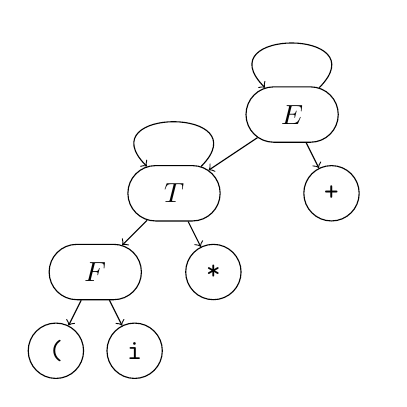
\begin{tikzpicture}
\tikzstyle{mono}=[draw,circle,minimum width=2em,font=\ttfamily];
\tikzstyle{con}=[draw,rounded rectangle,minimum height=2em,minimum width=4em];
\tikzstyle{dir}=[->];
\node [mono] (v2) at (-0.5,1.5) {(};
\node [mono] (v3) at (0.5,1.5) {i};
\node [con] (v1) at (0,2.5) {$F$};
\draw [dir] (v1) edge (v2);
\draw [dir] (v1) edge (v3);
\node [con] (v4) at (1,3.5) {$T$};
\draw [dir] (v4) edge (v1);
\node [mono] (v5) at (1.5,2.5) {*};
\draw [dir] (v4) edge (v5);
\draw [dir] (v4) edge[loop, looseness=4] (v4);
\node [con] (v6) at (2.5,4.5) {$E$};
\draw [dir] (v6) edge (v4);
\draw [dir] (v6) edge[loop, looseness=4] (v6);
\node [mono] (v7) at (3,3.5) {+};
\draw [dir] (v6) edge (v7);
\end{tikzpicture}